% Options for packages loaded elsewhere
\PassOptionsToPackage{unicode}{hyperref}
\PassOptionsToPackage{hyphens}{url}
%
\documentclass[
]{article}
\usepackage{lmodern}
\usepackage{amsmath}
\usepackage{ifxetex,ifluatex}
\ifnum 0\ifxetex 1\fi\ifluatex 1\fi=0 % if pdftex
  \usepackage[T1]{fontenc}
  \usepackage[utf8]{inputenc}
  \usepackage{textcomp} % provide euro and other symbols
  \usepackage{amssymb}
\else % if luatex or xetex
  \usepackage{unicode-math}
  \defaultfontfeatures{Scale=MatchLowercase}
  \defaultfontfeatures[\rmfamily]{Ligatures=TeX,Scale=1}
\fi
% Use upquote if available, for straight quotes in verbatim environments
\IfFileExists{upquote.sty}{\usepackage{upquote}}{}
\IfFileExists{microtype.sty}{% use microtype if available
  \usepackage[]{microtype}
  \UseMicrotypeSet[protrusion]{basicmath} % disable protrusion for tt fonts
}{}
\makeatletter
\@ifundefined{KOMAClassName}{% if non-KOMA class
  \IfFileExists{parskip.sty}{%
    \usepackage{parskip}
  }{% else
    \setlength{\parindent}{0pt}
    \setlength{\parskip}{6pt plus 2pt minus 1pt}}
}{% if KOMA class
  \KOMAoptions{parskip=half}}
\makeatother
\usepackage{xcolor}
\IfFileExists{xurl.sty}{\usepackage{xurl}}{} % add URL line breaks if available
\IfFileExists{bookmark.sty}{\usepackage{bookmark}}{\usepackage{hyperref}}
\hypersetup{
  pdftitle={Gestion de Portefeuille},
  pdfauthor={Berthoumieu Aymeric, Kingne Jéhoiakim et Jallouli Mouad},
  hidelinks,
  pdfcreator={LaTeX via pandoc}}
\urlstyle{same} % disable monospaced font for URLs
\usepackage[margin=1in]{geometry}
\usepackage{color}
\usepackage{fancyvrb}
\newcommand{\VerbBar}{|}
\newcommand{\VERB}{\Verb[commandchars=\\\{\}]}
\DefineVerbatimEnvironment{Highlighting}{Verbatim}{commandchars=\\\{\}}
% Add ',fontsize=\small' for more characters per line
\usepackage{framed}
\definecolor{shadecolor}{RGB}{248,248,248}
\newenvironment{Shaded}{\begin{snugshade}}{\end{snugshade}}
\newcommand{\AlertTok}[1]{\textcolor[rgb]{0.94,0.16,0.16}{#1}}
\newcommand{\AnnotationTok}[1]{\textcolor[rgb]{0.56,0.35,0.01}{\textbf{\textit{#1}}}}
\newcommand{\AttributeTok}[1]{\textcolor[rgb]{0.77,0.63,0.00}{#1}}
\newcommand{\BaseNTok}[1]{\textcolor[rgb]{0.00,0.00,0.81}{#1}}
\newcommand{\BuiltInTok}[1]{#1}
\newcommand{\CharTok}[1]{\textcolor[rgb]{0.31,0.60,0.02}{#1}}
\newcommand{\CommentTok}[1]{\textcolor[rgb]{0.56,0.35,0.01}{\textit{#1}}}
\newcommand{\CommentVarTok}[1]{\textcolor[rgb]{0.56,0.35,0.01}{\textbf{\textit{#1}}}}
\newcommand{\ConstantTok}[1]{\textcolor[rgb]{0.00,0.00,0.00}{#1}}
\newcommand{\ControlFlowTok}[1]{\textcolor[rgb]{0.13,0.29,0.53}{\textbf{#1}}}
\newcommand{\DataTypeTok}[1]{\textcolor[rgb]{0.13,0.29,0.53}{#1}}
\newcommand{\DecValTok}[1]{\textcolor[rgb]{0.00,0.00,0.81}{#1}}
\newcommand{\DocumentationTok}[1]{\textcolor[rgb]{0.56,0.35,0.01}{\textbf{\textit{#1}}}}
\newcommand{\ErrorTok}[1]{\textcolor[rgb]{0.64,0.00,0.00}{\textbf{#1}}}
\newcommand{\ExtensionTok}[1]{#1}
\newcommand{\FloatTok}[1]{\textcolor[rgb]{0.00,0.00,0.81}{#1}}
\newcommand{\FunctionTok}[1]{\textcolor[rgb]{0.00,0.00,0.00}{#1}}
\newcommand{\ImportTok}[1]{#1}
\newcommand{\InformationTok}[1]{\textcolor[rgb]{0.56,0.35,0.01}{\textbf{\textit{#1}}}}
\newcommand{\KeywordTok}[1]{\textcolor[rgb]{0.13,0.29,0.53}{\textbf{#1}}}
\newcommand{\NormalTok}[1]{#1}
\newcommand{\OperatorTok}[1]{\textcolor[rgb]{0.81,0.36,0.00}{\textbf{#1}}}
\newcommand{\OtherTok}[1]{\textcolor[rgb]{0.56,0.35,0.01}{#1}}
\newcommand{\PreprocessorTok}[1]{\textcolor[rgb]{0.56,0.35,0.01}{\textit{#1}}}
\newcommand{\RegionMarkerTok}[1]{#1}
\newcommand{\SpecialCharTok}[1]{\textcolor[rgb]{0.00,0.00,0.00}{#1}}
\newcommand{\SpecialStringTok}[1]{\textcolor[rgb]{0.31,0.60,0.02}{#1}}
\newcommand{\StringTok}[1]{\textcolor[rgb]{0.31,0.60,0.02}{#1}}
\newcommand{\VariableTok}[1]{\textcolor[rgb]{0.00,0.00,0.00}{#1}}
\newcommand{\VerbatimStringTok}[1]{\textcolor[rgb]{0.31,0.60,0.02}{#1}}
\newcommand{\WarningTok}[1]{\textcolor[rgb]{0.56,0.35,0.01}{\textbf{\textit{#1}}}}
\usepackage{graphicx}
\makeatletter
\def\maxwidth{\ifdim\Gin@nat@width>\linewidth\linewidth\else\Gin@nat@width\fi}
\def\maxheight{\ifdim\Gin@nat@height>\textheight\textheight\else\Gin@nat@height\fi}
\makeatother
% Scale images if necessary, so that they will not overflow the page
% margins by default, and it is still possible to overwrite the defaults
% using explicit options in \includegraphics[width, height, ...]{}
\setkeys{Gin}{width=\maxwidth,height=\maxheight,keepaspectratio}
% Set default figure placement to htbp
\makeatletter
\def\fps@figure{htbp}
\makeatother
\setlength{\emergencystretch}{3em} % prevent overfull lines
\providecommand{\tightlist}{%
  \setlength{\itemsep}{0pt}\setlength{\parskip}{0pt}}
\setcounter{secnumdepth}{-\maxdimen} % remove section numbering
\usepackage[utf8]{inputenc}
\usepackage{booktabs}
\usepackage{longtable}
\usepackage{array}
\usepackage{multirow}
\usepackage{wrapfig}
\usepackage{float}
\usepackage{colortbl}
\usepackage{pdflscape}
\usepackage{tabu}
\usepackage{threeparttable}
\usepackage{threeparttablex}
\usepackage[normalem]{ulem}
\usepackage{makecell}
\usepackage{xcolor}
\ifluatex
  \usepackage{selnolig}  % disable illegal ligatures
\fi

\title{Gestion de Portefeuille}
\usepackage{etoolbox}
\makeatletter
\providecommand{\subtitle}[1]{% add subtitle to \maketitle
  \apptocmd{\@title}{\par {\large #1 \par}}{}{}
}
\makeatother
\subtitle{TP-3: Modèle à un facteur et modèle de Treynor Black}
\author{Berthoumieu Aymeric, Kingne Jéhoiakim et Jallouli Mouad}
\date{Février-Mars 2020}

\begin{document}
\maketitle

\hypertarget{donnuxe9es}{%
\section{Données}\label{donnuxe9es}}

\hypertarget{suxe9ries-de-rendement-mensuel-pour-11-valeurs}{%
\subsection{Séries de rendement mensuel pour 11
valeurs:}\label{suxe9ries-de-rendement-mensuel-pour-11-valeurs}}

\begin{Shaded}
\begin{Highlighting}[]
\NormalTok{monthly.ret.file }\OtherTok{\textless{}{-}} \StringTok{"./monthly.ret.rda"}
\FunctionTok{load}\NormalTok{(monthly.ret.file)}
\FunctionTok{index}\NormalTok{(monthly.ret) }\OtherTok{\textless{}{-}} \FunctionTok{floor\_date}\NormalTok{(}\FunctionTok{index}\NormalTok{(monthly.ret), }\StringTok{"month"}\NormalTok{)}
\end{Highlighting}
\end{Shaded}

\hypertarget{matrice-de-covariance-des-rendements}{%
\subsection{Matrice de covariance des
rendements:}\label{matrice-de-covariance-des-rendements}}

\begin{Shaded}
\begin{Highlighting}[]
\FunctionTok{kable}\NormalTok{(}\FunctionTok{cov}\NormalTok{(monthly.ret), }\AttributeTok{booktabs=}\NormalTok{T) }\SpecialCharTok{\%\textgreater{}\%}
\FunctionTok{kable\_styling}\NormalTok{(}\AttributeTok{latex\_options=}\FunctionTok{c}\NormalTok{(}\StringTok{"scale\_down"}\NormalTok{, }\StringTok{"HOLD\_position"}\NormalTok{))}
\end{Highlighting}
\end{Shaded}

\begin{table}[H]
\centering
\resizebox{\linewidth}{!}{
\begin{tabular}{lrrrrrrrrrrr}
\toprule
  & AAPL & AMZN & MSFT & F & SPY & QQQ & XOM & MMM & HD & PG & KO\\
\midrule
AAPL & 0.0079015 & 0.0035933 & 0.0028724 & 0.0036506 & 0.0021193 & 0.0033242 & 0.0012183 & 0.0019158 & 0.0012159 & 0.0009073 & 0.0009576\\
AMZN & 0.0035933 & 0.0097937 & 0.0026625 & 0.0025940 & 0.0020258 & 0.0030033 & 0.0011468 & 0.0016726 & 0.0016066 & 0.0003831 & 0.0013968\\
MSFT & 0.0028724 & 0.0026625 & 0.0044949 & 0.0032132 & 0.0017774 & 0.0022969 & 0.0009976 & 0.0012898 & 0.0015753 & 0.0007414 & 0.0011363\\
F & 0.0036506 & 0.0025940 & 0.0032132 & 0.0226257 & 0.0032869 & 0.0034954 & 0.0017697 & 0.0034663 & 0.0032642 & 0.0014660 & 0.0014993\\
SPY & 0.0021193 & 0.0020258 & 0.0017774 & 0.0032869 & 0.0017549 & 0.0019207 & 0.0012159 & 0.0016906 & 0.0015105 & 0.0008284 & 0.0009008\\
\addlinespace
QQQ & 0.0033242 & 0.0030033 & 0.0022969 & 0.0034954 & 0.0019207 & 0.0025159 & 0.0010479 & 0.0016973 & 0.0016125 & 0.0007561 & 0.0008650\\
XOM & 0.0012183 & 0.0011468 & 0.0009976 & 0.0017697 & 0.0012159 & 0.0010479 & 0.0025213 & 0.0015076 & 0.0008121 & 0.0006409 & 0.0007365\\
MMM & 0.0019158 & 0.0016726 & 0.0012898 & 0.0034663 & 0.0016906 & 0.0016973 & 0.0015076 & 0.0032027 & 0.0016559 & 0.0009968 & 0.0008642\\
HD & 0.0012159 & 0.0016066 & 0.0015753 & 0.0032642 & 0.0015105 & 0.0016125 & 0.0008121 & 0.0016559 & 0.0037458 & 0.0005615 & 0.0005566\\
PG & 0.0009073 & 0.0003831 & 0.0007414 & 0.0014660 & 0.0008284 & 0.0007561 & 0.0006409 & 0.0009968 & 0.0005615 & 0.0018508 & 0.0009004\\
\addlinespace
KO & 0.0009576 & 0.0013968 & 0.0011363 & 0.0014993 & 0.0009008 & 0.0008650 & 0.0007365 & 0.0008642 & 0.0005566 & 0.0009004 & 0.0019550\\
\bottomrule
\end{tabular}}
\end{table}

\hypertarget{rendement-moyen-mensuel}{%
\subsection{Rendement moyen mensuel}\label{rendement-moyen-mensuel}}

\begin{Shaded}
\begin{Highlighting}[]
\FunctionTok{kable}\NormalTok{(}\FunctionTok{t}\NormalTok{(}\FunctionTok{colMeans}\NormalTok{(monthly.ret)), }\AttributeTok{booktabs=}\NormalTok{T,  }
      \AttributeTok{caption=}\StringTok{"Rendement moyen mensuel"}\NormalTok{) }\SpecialCharTok{\%\textgreater{}\%}
\FunctionTok{kable\_styling}\NormalTok{(}\AttributeTok{latex\_options=}\FunctionTok{c}\NormalTok{(}\StringTok{"scale\_down"}\NormalTok{,}\StringTok{"HOLD\_position"}\NormalTok{))}
\end{Highlighting}
\end{Shaded}

\begin{table}[H]

\caption{\label{tab:unnamed-chunk-3}Rendement moyen mensuel}
\centering
\resizebox{\linewidth}{!}{
\begin{tabular}[t]{rrrrrrrrrrr}
\toprule
AAPL & AMZN & MSFT & F & SPY & QQQ & XOM & MMM & HD & PG & KO\\
\midrule
0.0254037 & 0.0298355 & 0.0151864 & 0.0115177 & 0.0075856 & 0.0122593 & 0.0016595 & 0.0079299 & 0.0151356 & 0.0073821 & 0.0100164\\
\bottomrule
\end{tabular}}
\end{table}

\hypertarget{taux-sans-risque}{%
\subsection{Taux sans risque}\label{taux-sans-risque}}

Le taux sans risque mensuel est obtenu de la Réserve Fédérale US. A
diviser par 12 pour être cohérent avec les rendement des titres.

\begin{Shaded}
\begin{Highlighting}[]
\NormalTok{tmp }\OtherTok{\textless{}{-}} \FunctionTok{read.csv}\NormalTok{(}\StringTok{"DP\_LIVE\_01032020211755676.csv"}\NormalTok{, }\AttributeTok{header=}\ConstantTok{TRUE}\NormalTok{, }\AttributeTok{sep=}\StringTok{";"}\NormalTok{)[, }\FunctionTok{c}\NormalTok{(}\StringTok{"TIME"}\NormalTok{, }\StringTok{"Value"}\NormalTok{)]}
\NormalTok{dt }\OtherTok{\textless{}{-}} \FunctionTok{ymd}\NormalTok{(}\FunctionTok{paste}\NormalTok{(tmp}\SpecialCharTok{$}\NormalTok{TIME, }\StringTok{"{-}01"}\NormalTok{, }\AttributeTok{sep=}\StringTok{""}\NormalTok{))}
\NormalTok{rf\_rate }\OtherTok{\textless{}{-}} \FunctionTok{xts}\NormalTok{((tmp}\SpecialCharTok{$}\NormalTok{Value}\SpecialCharTok{/}\FloatTok{100.0}\NormalTok{)}\SpecialCharTok{/}\DecValTok{12}\NormalTok{, dt)}
\FunctionTok{colnames}\NormalTok{(rf\_rate) }\OtherTok{\textless{}{-}} \StringTok{"Rf"}
\NormalTok{monthly.ret}\FloatTok{.2} \OtherTok{\textless{}{-}} \FunctionTok{merge.xts}\NormalTok{(monthly.ret, rf\_rate, }\AttributeTok{join=}\StringTok{"inner"}\NormalTok{)}
\end{Highlighting}
\end{Shaded}

\begin{figure}
\centering
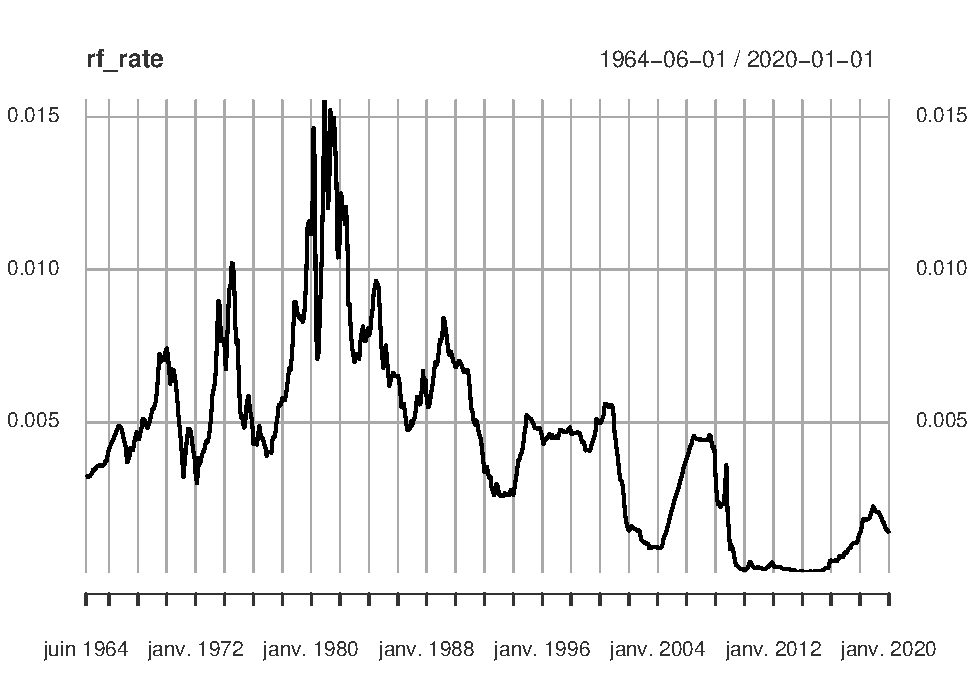
\includegraphics{TP-3_files/figure-latex/unnamed-chunk-5-1.pdf}
\caption{taux sans risque mensuel}
\end{figure}

\hypertarget{estimation-dun-moduxe8le-uxe0-un-facteur}{%
\section{Estimation d'un modèle à un
facteur}\label{estimation-dun-moduxe8le-uxe0-un-facteur}}

\begin{itemize}
\tightlist
\item
  Utiliser l'indice SPY comme proxy pour le marché et estimer pour
  chaque titre le modèle:
\end{itemize}

\[
R_i(t) - R_f(t) = \alpha + \beta (R_M(t) - R_f(t)) + \epsilon(t)
\] en utilisant la fonction \texttt{lm}. - Placer chaque titre sur un
diagramme rendement/beta et calculer par regression la droite de marché
des titres risqués. - En déduire les titres qui, selon ce modèle,
\emph{semblent} chers et ceux qui semblent sous-évalués.

Est-ce que ces mesures de cherté relative vous semblent correctes?
Essayez de mesurer la robustesse de ce calcul en estimant le modèles sur
des sous-intervalles de temps.

Présentez vos résultats de manière synthétique.

\begin{Shaded}
\begin{Highlighting}[]
\FunctionTok{kable}\NormalTok{(df, }\AttributeTok{booktabs=}\NormalTok{T, }\AttributeTok{caption=}\StringTok{"Alpha and beta by asset"}\NormalTok{) }\SpecialCharTok{\%\textgreater{}\%}
    \FunctionTok{kable\_styling}\NormalTok{(}\AttributeTok{latex\_options=}\FunctionTok{c}\NormalTok{(}\StringTok{"scale\_down"}\NormalTok{,}\StringTok{"HOLD\_position"}\NormalTok{))}
\end{Highlighting}
\end{Shaded}

\begin{table}[H]

\caption{\label{tab:unnamed-chunk-7}Alpha and beta by asset}
\centering
\resizebox{\linewidth}{!}{
\begin{tabular}[t]{lrrrrrrrrrrrr}
\toprule
  & AAPL & AMZN & MSFT & F & SPY & QQQ & XOM & MMM & HD & PG & KO & Rf\\
\midrule
alpha & 0.0167401 & 0.0212874 & 0.0073307 & -0.0008543 & 0 & 0.0039254 & -0.0031066 & 0.0007451 & 0.0080456 & 0.0034204 & 0.0056304 & 0\\
beta & 1.1948376 & 1.1465481 & 1.0148488 & 1.8508513 & 1 & 1.0959372 & 0.6751296 & 0.9608010 & 0.8746106 & 0.4693130 & 0.5136098 & 0\\
\bottomrule
\end{tabular}}
\end{table}

On remarque que SPY a bien un alpha de 0 et un beta de 1 ce qui est
attendu puisqu'il est pris comme référence (assimilé au marché).

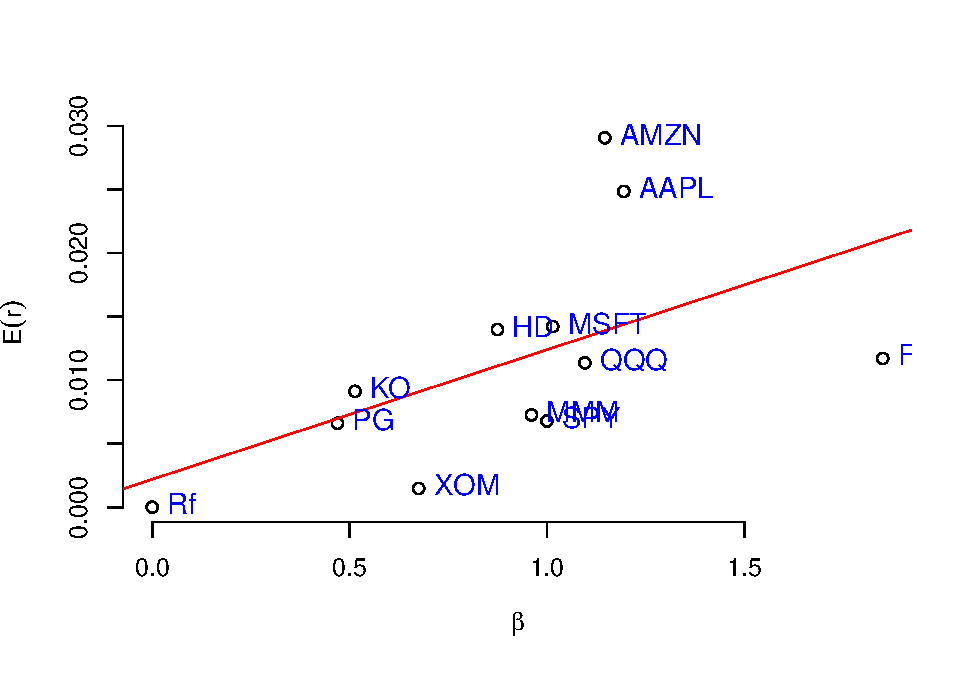
\includegraphics{TP-3_files/figure-latex/unnamed-chunk-8-1.pdf}

\begin{itemize}
\item
  Il est intéressant de remarquer que le SnP500 n'est pas sur la droite
  de marchés des titres. Cela est dû au fait que ce soit une régression
  équipondérée sur les quelques titres proposés ici. Si nous voulions
  l'intégrer à la droite, il faudrait prendre tous les titres de
  l'indice et faire une régression pondérée par les poids de l'indice.
\item
  Comme prévu, les actions AMZN, AAPL ont des betas bien supérieurs à 1:
  ils sont très corrélés au SPY mais ils sont aussi très volatile. Elles
  peuvent surperformer le SPY dans un bullish market, mais en
  contrepartie leur perte serait aussi plus importante dans le cas d'un
  bearish market. Cette capacité à surperformer se reflète aussi sur
  leurs alphas respectifs qui sont postifs et plus importants par
  rapport au reste. Des actions comme MSFT, QQQ et MMM sont
  raisonnablement corrélés (beta \textasciitilde1) avec le marché SPY:
  elles suivent les tendances du marché mais d'une manière moins
  volatile.
\item
  Una action comme Ford (F) a également un beta bien supérieur à 1, elle
  est donc très volatile et susceptible de surperformer le marché.
  Cependant, on voit qu'elle a un alpha négatif très faible:
  contrairement aux attentes elle a sousperformer historiquement le
  marché. Un investissement dans cette action a généré un rendement qui
  n'a pas compensé le risque de volatilité assumé, donc elle devrait
  être surévaluée.
\item
  Donc des actions comme AMZN, AAPL rajoutent plus de volatilité à un
  portefeuille mais un potentiel de gain plus important aussi. Des
  actions comme KO et PG qui sont moins corrélés (faible beta
  \textless{} 1) au marché sont aussi moins volatile et les rajouter à
  notre portefeuille le rend moins risqué mais ça réduit aussi le
  potentiel du gain.
\item
  Ainsi, en première approche, des titres comme AAPL, AMZN, KO, HD et
  MSFT semblent sous-cotés (suivant différtentes proportions), et cela,
  de manière très forte pour les deux premiers. A l'inverse, XOM, F, MMM
  et même SPY (le marché) semblent trop chers.
\item
  Cependant, d'après les tests statistiques de la fonction lm, les
  \(\alpha\) de KO, MSFT pour les sous-côtés et de XOM, F, MMM, SPY pour
  les sur-côtés ne sont pas significatifs.
\item
  De plus, si l'on se concentre seulement sur les deux dernières années
  ( fixant starting.mont à dim(monthly.ret.2){[}1{]}-24), les \(\alpha\)
  de AAPL et de AMZN sont aussi non significatifs.
\end{itemize}

\hypertarget{moduxe8le-de-treynor-black}{%
\section{Modèle de Treynor-Black}\label{moduxe8le-de-treynor-black}}

Le modèle de Treynor-Black a pour objectif d'exploiter les informations
calculées en première partie. L'idée étant de constituer un portefeuille
``actif'' avec les titres qui semblent mal valorisés par le marché, et
allouer le reste de sa richesse au portefeuille de marché.

\hypertarget{selection-des-titres-uxe0-inclure-dans-le-portefeuille-actif.}{%
\subsection{Selection des titres à inclure dans le portefeuille
actif.}\label{selection-des-titres-uxe0-inclure-dans-le-portefeuille-actif.}}

C'est l'étape délicate de la méthode de Treynor-Black. A partir de
l'évaluation du modèle à un facteur, déterminez quels titres méritent de
figurer dans le portefeuille actif. En théorie, on a envie d'acheter les
titres sous-cotés (\(\alpha_i > 0\)) mais cette anomalie n'est peut être
qu'apparente! Il faut également apprécier la qualité de l'estimation
statistique.

En testant diverses combinaisons de titres à mettre dans le portefeuille
actif, vous pourrez mesurer la sensibilité de modèle de Treynor-Black
aux données.

\hypertarget{duxe9termination-du-portefeuille-actif}{%
\subsection{Détermination du portefeuille
actif}\label{duxe9termination-du-portefeuille-actif}}

Ayant choisi les titres à inclure dans le portefeuille actif, on
rappelle que le poids de chaque titre dans le portefeuille actif est
proportionnel au ratio \(\alpha_i/\sigma^2(\epsilon_i)\):

\[
w_i = \frac{\alpha_i/\sigma^2(\epsilon_i)}{\sum_i \alpha_i/\sigma^2(\epsilon_i)}
\]

Calculer les poids des actifs dans le portefeuille actif. Justifier
votre choix d'inclure ou d'exclure tel ou tel instrument.

Calculez les valeurs suivantes concernant le portefeuille actif:

\begin{description}
\item[$R_A$] Excess de rendement
\item[$\alpha_A$] alpha du portefeuille actif
\item[$\beta_A$]  beta du portefeuille actif
\item[$\sigma_A$] ecart-type du portefeuille actif
\item[$\sigma^2(e_A)$] variance résiduelle du portefeuille actif

\end{description}

\hypertarget{commentaire-sur-le-choix-des-actifs}{%
\subsubsection{Commentaire sur le choix des
actifs}\label{commentaire-sur-le-choix-des-actifs}}

On choisit des titre pas trop risqués (\(\beta\) \textless{} 1) avec des
\(\alpha\) différents de 0 afin d'arbitrer les miss-pricing du marché.

\begin{table}[H]

\caption{\label{tab:unnamed-chunk-9}weight by asset}
\centering
\begin{tabular}[t]{lrrr}
\toprule
  & KO & HD & XOM\\
\midrule
specific risk² & 0.0015006 & 0.0024247 & 0.0016176\\
weight\_n & 0.7285937 & 0.6443480 & -0.3729418\\
beta & 0.5136098 & 0.8746106 & 0.6751296\\
alpha & 0.0056304 & 0.0080456 & -0.0031066\\
\bottomrule
\end{tabular}
\end{table}

\begin{itemize}
\tightlist
\item
  Plus la valeur \(\beta\) de l'actif est faible plus il est un bon
  diversificateur et plus son allocation est importante. Cependant, un
  grand ``specific risk'' vient pénaliser l'allocation de l'actif en
  réduisant son poids correspondant.
\item
  Par contre, plus l'actif est ``bon marché'' selon le modèle
  (\(\alpha\) grand), plus son poids sera important. En effet,
  \(\alpha\) représente une anomalie de pricing. On s'attend donc à ce
  que le marché corrige cette anomalie et remontant le prix de l'actif
  et on veut en profiter. On vient donc faire cet ``arbitrage''.
\item
  Ainsi les poids sont une combinaison du potentiel gain à faire en
  profitant de l'anomalie de marché rapporté au risque que cela implique
  de détenir ce titre.
\end{itemize}

\hypertarget{statistique-du-portefeuille-actif}{%
\subsubsection{Statistique du portefeuille
actif}\label{statistique-du-portefeuille-actif}}

\begin{verbatim}
## [1] "The excess return is :  1.51 %"
\end{verbatim}

\begin{verbatim}
## [1] "The Active Portfolio Alpha is :  0.01"
\end{verbatim}

\begin{verbatim}
## [1] "The Active Portfolio Beta is :  0.69"
\end{verbatim}

\begin{verbatim}
## [1] "The Active Portfolio standard deviation is :  5.18 %"
\end{verbatim}

\begin{verbatim}
## [1] "The Active Portfolio residual variance is :  4.11407e-06"
\end{verbatim}

\hypertarget{duxe9termination-de-la-ponduxe9ration-entre-le-portefeuille-actif-et-le-portefeuille-de-marchuxe9.}{%
\subsection{Détermination de la pondération entre le portefeuille actif
et le portefeuille de
marché.}\label{duxe9termination-de-la-ponduxe9ration-entre-le-portefeuille-actif-et-le-portefeuille-de-marchuxe9.}}

On rappelle l'allocation de richesse au portefeuille actif:

\[
w_A = \frac{\alpha_A \sigma^2_M}{\alpha_A \sigma^2_M (1-\beta_A) + R_M \sigma^2(e_A)}
\]

Avec:

\[
\begin{aligned}
R_A & = \alpha_A + \beta_A R_M \\
\sigma^2_A & = \beta^2_A \sigma^2_M + \sigma^2(e_A)
\end{aligned}
\]

\begin{verbatim}
## [1] "Accordiding to the Treynor's Model, the active portfolio contribution is :  316.681061530475 %"
\end{verbatim}

\hypertarget{comentaire}{%
\subsubsection{Comentaire}\label{comentaire}}

Le modèle affacte un poids démesuré au portefeuille car il ne le
considère pas trop risqué (\(\beta\) \textless{} 1) et veut profiter des
corrections de marchés sur les \(\alpha\) positifs (position long sur
ces assets) et négatif (position short).

\hypertarget{capital-allocation-line}{%
\subsection{Capital Allocation Line}\label{capital-allocation-line}}

Calculez l'espérance de rendement et le risque de quelques portefeuilles
situés sur la ``Capital Allocation Line'' qui joint l'actif sans risque
et le portefeuille tangent. Placez la solution du modèle de
Treynor-Black, le portefeuille actif et le portefeuille de marché sur le
graphique ci-dessous.

\begin{Shaded}
\begin{Highlighting}[]
\NormalTok{Assets }\OtherTok{\textless{}{-}} \FunctionTok{c}\NormalTok{(}\StringTok{"AAPL"}\NormalTok{, }\StringTok{"AMZN"}\NormalTok{, }\StringTok{"MSFT"}\NormalTok{, }\StringTok{"F"}\NormalTok{,  }\StringTok{"XOM"}\NormalTok{, }\StringTok{"MMM"}\NormalTok{,  }\StringTok{"HD"}\NormalTok{,   }\StringTok{"PG"}\NormalTok{,   }\StringTok{"KO"}\NormalTok{)}
\NormalTok{plot.data }\OtherTok{\textless{}{-}}\NormalTok{ monthly.ret}\FloatTok{.3}\NormalTok{[, }\FunctionTok{c}\NormalTok{(Assets, }\StringTok{"Rf"}\NormalTok{)]}
\ControlFlowTok{for}\NormalTok{(a }\ControlFlowTok{in}\NormalTok{ Assets) \{}
\NormalTok{  plot.data[, a] }\OtherTok{\textless{}{-}}\NormalTok{ plot.data[, a] }\SpecialCharTok{{-}}\NormalTok{ plot.data}\SpecialCharTok{$}\NormalTok{Rf}
\NormalTok{  \}}

\NormalTok{res }\OtherTok{\textless{}{-}} \FunctionTok{data.frame}\NormalTok{(}\AttributeTok{Mean=}\FunctionTok{apply}\NormalTok{(plot.data[, Assets],}\DecValTok{2}\NormalTok{,mean),}
                  \AttributeTok{Sd =} \FunctionTok{apply}\NormalTok{(plot.data[, Assets],}\DecValTok{2}\NormalTok{,sd))}
\FunctionTok{rownames}\NormalTok{(res) }\OtherTok{\textless{}{-}}\NormalTok{ Assets}
\end{Highlighting}
\end{Shaded}

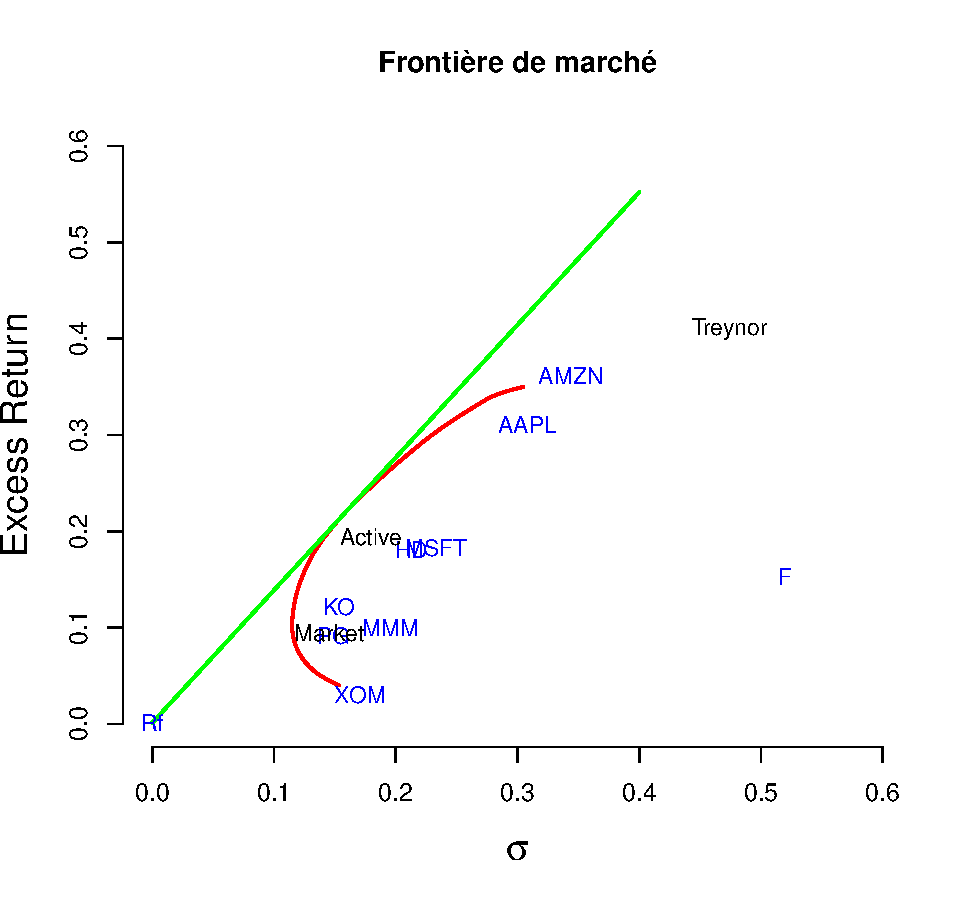
\includegraphics{TP-3_files/figure-latex/unnamed-chunk-14-1.pdf}

\hypertarget{commentaires}{%
\subsubsection{Commentaires}\label{commentaires}}

On remarque que, assez adroitement, le portefeuille actif est plus
proche du portefeuille tangent que ne l'est le marché (donc plus optimal
selon le modèle MV). Par ailleurs, le portefeuille de Treynor qui est
sensé profiter des miss-pricing du marché reste plus risqué pour son
espérance de rendement que l'optimum.

\end{document}
